\documentclass[tikz,border=2pt]{standalone}
\usepackage{amsmath}
\usepackage{amssymb}
\usepackage{pgfplots}
\pgfplotsset{compat=1.18}
\usetikzlibrary{arrows.meta}
\begin{document}
% Table 5.2: max <-> min; constraints of the max problem (>=, <=, =) <-> variables of the min problem (<=0, >=0, free);
% variables of the max problem (>=0, <=0, free) <-> constraints of the min problem (>=, <=, =).
% Green: the two standard-form pairs of Table 5.1 (<= gives >=0, >=0 gives >=).
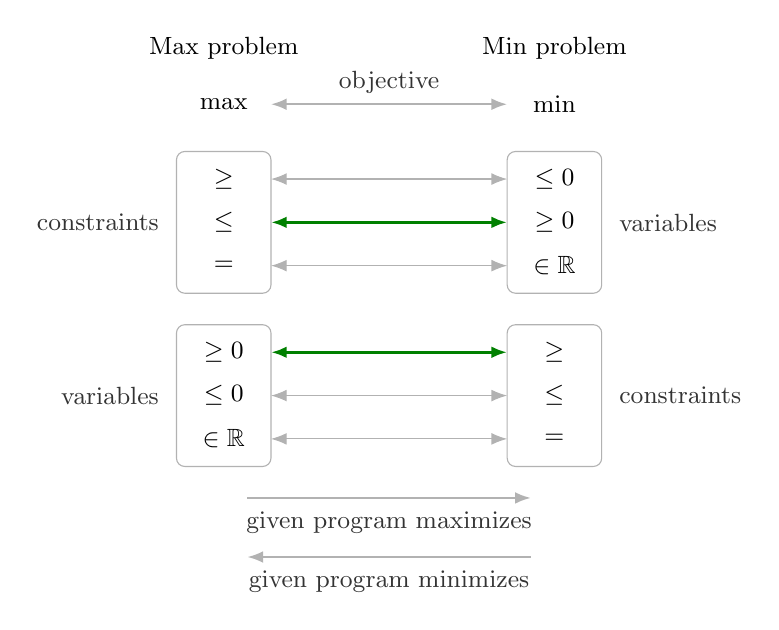
\begin{tikzpicture}[font=\small, >={Latex[length=2mm]}]
  % headers
  \node[anchor=south] at (0,0.45) {Max problem};
  \node[anchor=south] at (4.2,0.45) {Min problem};
  % objective row
  \node at (0,0) {$\max$};
  \node at (4.2,0) {$\min$};
  \draw[gray!60, <->, thick] (0.6,0) -- (3.6,0);
  \node[gray!40!black, anchor=south] at (2.1,0.02) {objective};
  % group frames
  \draw[gray!60, rounded corners=3pt] (-0.6,-0.6) rectangle (0.6,-2.4);
  \draw[gray!60, rounded corners=3pt] (3.6,-0.6) rectangle (4.8,-2.4);
  \draw[gray!60, rounded corners=3pt] (-0.6,-2.8) rectangle (0.6,-4.6);
  \draw[gray!60, rounded corners=3pt] (3.6,-2.8) rectangle (4.8,-4.6);
  \node[gray!40!black, anchor=east] at (-0.7,-1.5) {constraints};
  \node[gray!40!black, anchor=west] at (4.9,-1.5) {variables};
  \node[gray!40!black, anchor=east] at (-0.7,-3.7) {variables};
  \node[gray!40!black, anchor=west] at (4.9,-3.7) {constraints};
  % constraints of the max problem <-> variables of the min problem
  \node at (0,-0.95) {$\geq$};      \node at (4.2,-0.95) {$\leq0$};
  \node at (0,-1.5) {$\leq$};       \node at (4.2,-1.5) {$\geq0$};
  \node at (0,-2.05) {$=$};         \node at (4.2,-2.05) {$\in\mathbb{R}$};
  \draw[gray!60, <->] (0.6,-0.95) -- (3.6,-0.95);
  \draw[green!50!black, <->, very thick] (0.6,-1.5) -- (3.6,-1.5);
  \draw[gray!60, <->] (0.6,-2.05) -- (3.6,-2.05);
  % variables of the max problem <-> constraints of the min problem
  \node at (0,-3.15) {$\geq0$};     \node at (4.2,-3.15) {$\geq$};
  \node at (0,-3.7) {$\leq0$};      \node at (4.2,-3.7) {$\leq$};
  \node at (0,-4.25) {$\in\mathbb{R}$}; \node at (4.2,-4.25) {$=$};
  \draw[green!50!black, <->, very thick] (0.6,-3.15) -- (3.6,-3.15);
  \draw[gray!60, <->] (0.6,-3.7) -- (3.6,-3.7);
  \draw[gray!60, <->] (0.6,-4.25) -- (3.6,-4.25);
  % reading directions
  \draw[gray!60, ->, thick] (0.3,-5.0) -- (3.9,-5.0);
  \node[gray!40!black, anchor=north] at (2.1,-5.05) {given program maximizes};
  \draw[gray!60, ->, thick] (3.9,-5.75) -- (0.3,-5.75);
  \node[gray!40!black, anchor=north] at (2.1,-5.8) {given program minimizes};
\end{tikzpicture}
\end{document}
